% =======================================================================
%
%                                SETUP
%
% =======================================================================

\documentclass[12pt, oneside]{article}
\usepackage[utf8]{inputenc}
\usepackage[IL2, T1]{fontenc}
\usepackage{hyperref} 
\usepackage[czech, english]{babel}
\usepackage{graphicx}
\graphicspath{ {./static/} }
\usepackage{geometry}
\geometry{
	left=2cm,
	top=3cm,
	right=2cm,
	bottom=3cm
}
\usepackage{tcolorbox}
\usepackage{lipsum}
\usepackage{float}
\usepackage{caption}
\captionsetup[figure]{labelformat=empty}

\pagenumbering{gobble}
\setlength{\parskip}{1em}

% =======================================================================
%
%                                CUSTOM OBJECTS
%
% =======================================================================

\newtcolorbox{roundexBox}{
  colback=white,        % Background color
  colframe=black,       % Border color
  boxrule=0.8mm,        % Border thickness
  arc=6mm,              % Radius of the rounded corners
  auto outer arc,       % Apply the arc radius to the outer corners
  width=0.8\textwidth  % Width of the box
}

% =======================================================================
%
%                                CONTENT
%
% =======================================================================

\begin{document}

\thispagestyle{empty}
\begin{center}
	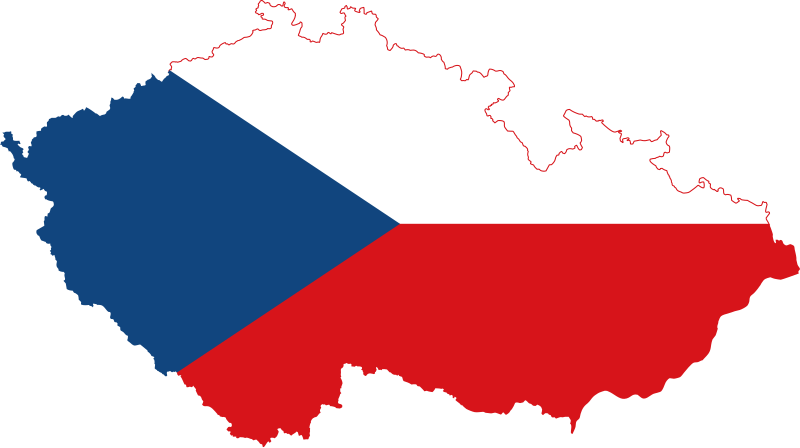
\includegraphics[width=10cm]{map.png}
	
  \vspace*{4em}

  \rule{\linewidth}{0.5mm}
  \vspace*{1em}
  
  {\LARGE Czechia – a thorough Geoguessr guide} \\ [1cm]
	\textbf{\Large Marek Smolík}
  \\ \texttt{spalovac\_mrtvol@discord}
  \\ \texttt{\href{https://github.com/dynamo58}{GitHub}}
  \\ \texttt{\href{https://www.twitch.tv/bigladmush22}{Twitch profile}}
  \\ \texttt{\href{https://www.geoguessr.com/user/5ee78ead03f80c500c7cba22}{Geoguessr profile}}
  \vspace*{1em}
  \\ Last edited:\ \today
  \\ Version:\ \texttt{0.0}


  \vspace*{1em}
  \rule{\linewidth}{0.5mm}
\end{center}

\newpage

\tableofcontents

\newpage

\begin{abstract}
Czechia or the Czech republic is a country notoriously difficult. For one thing it is very difficult to region-guess and at times also to distinguish from some of the surrounding countries. This document tries to outline all of the possible metas and actual geography knowledge there is to be obtain in order to guess this country accuretly and be able to make informed region-guesses within the country itself.
\end{abstract}

\clearpage

\pagenumbering{arabic}
\setcounter{page}{1}

\section{Introduction}

\subsection{About the author}

My name is Marek Smolík and I am a fellow Geoguessr player. I have lived in Czechia my whole life and played Czechia extensively on Geoguessr, speedrunning it among other gamemodes. As such I have accumulated knowledge that is not necessarily well-known. I have no intention in trying to gatekeep this information... the complete opposite... actually.

\subsection{Contribution}

All types of contribution to this doc are welcome. Contribution may include a suggestion, a dispute of correctness about something included, etc. If you wish to contribute to this document you can do so through any of the on the title page. Preferred way is opening an issue on \href{https://github.com/dynamo58/geoguessr-czechia-guide}{this doc's GitHub page} or outright opening a pull request. But getting hang of me on any of the other platforms is also fine. All the contribees will be included in the \hyperref[sec:ack]{Acknowledgements section} if they choose so.

\newpage
\section{Recognizing the country}
Czechia can come to resemble pretty much all of it's neighbors, as well as France and on the off-shoot some like some of its east and south-east European co-inhabitants.

\subsection{Language}
Czechia has the Czech language as it's one and only official language. It is pretty easy to distinguish it from languages such as German, French or Hungarian, but majority of Slavic languages, especially those being written usign the Latin script will be tough to distinguish. 

\begin{itemize}
  \item \textbf{Characters unique solely to Czech:} ř/Ř
  \item \textbf{Characters in Czech but not in Slovak:} ů/Ů, ř/Ř
  \item \textbf{Characters in Slovak but not in Czech:} ä/Ä, ŕ/Ŕ, ĺ/Ĺ, ľ/Ľ
  \item \textbf{Characters in Czech but not in Polish:} ů/Ů, ú/Ú, ř/Ř, č/Č, ď/Ď, ě/Ě, é/É, š/Š, í/Í, ý/Ý, ž/Ž
  \item \textbf{Characters in Polish but not in Czech:} ż/Ż, ź/Ź, ś/Ś, ń/Ń, ł/Ł, ę/Ę, ć/Ć, ą/Ą
\end{itemize}

Additionally Polish uses the letter \textit{w}/\textit{W} extensivelly while in Czech it is very rare and used exclusively in loanwords.

Example of Czech text:
\begin{center} \begin{roundexBox}
  Každý má právo na vzdělání. Vzdělání nechť je bezplatné, alespoň v počátečních a základních stupních. Základní vzdělání je povinné. Technické a odborné vzdělání budiž všeobecně přístupné a rovněž vyšší vzdělání má být stejně přístupné všem podle schopností. Vzdělání má směřovat k plnému rozvoji lidské osobnosti a k posílení úcty k lidským právům a základním svobodám.
\end{roundexBox} \end{center}

Example of Polish text:
\begin{center} \begin{roundexBox}
  Każdy człowiek ma prawo do nauki. Nauka jest bezpłatna, przynajmniej na stopniu podstawowym. Nauka podstawowa jest obowiązkowa. Oświata techniczna i zawodowa jest powszechnie dostępna, a studia wyższe są dostępne dla wszystkich na zasadzie równości w zależności od zalet osobistych. Celem nauczania jest pełny rozwój osobowości ludzkiej i ugruntowanie poszanowania praw człowieka i podstawowych wolności.
\end{roundexBox} \end{center}

Example of Slovak text:
\begin{center} \begin{roundexBox}
  Každý má právo na vzdelanie. Vzdelanie nech je bezplatné aspoň v začiatočných a základných stupňoch. Základné vzdelanie je povinné. Technické a odborné vzdelanie nech je všeobecne prístupné a vyššie vzdelanie má byť rovnako prístupné každému podľa jeho schopností. Vzdelanie má smerovať k plnému rozvoju ľudskej osobnosti a k posilneniu úcty k ľudským právam a základným slobodám.
\end{roundexBox} \end{center}


\subsection{Topography}
Before we start here we will need the political map showing us the regions of Czechia so that we can refer to them later on via their names:

\begin{figure}[H]
  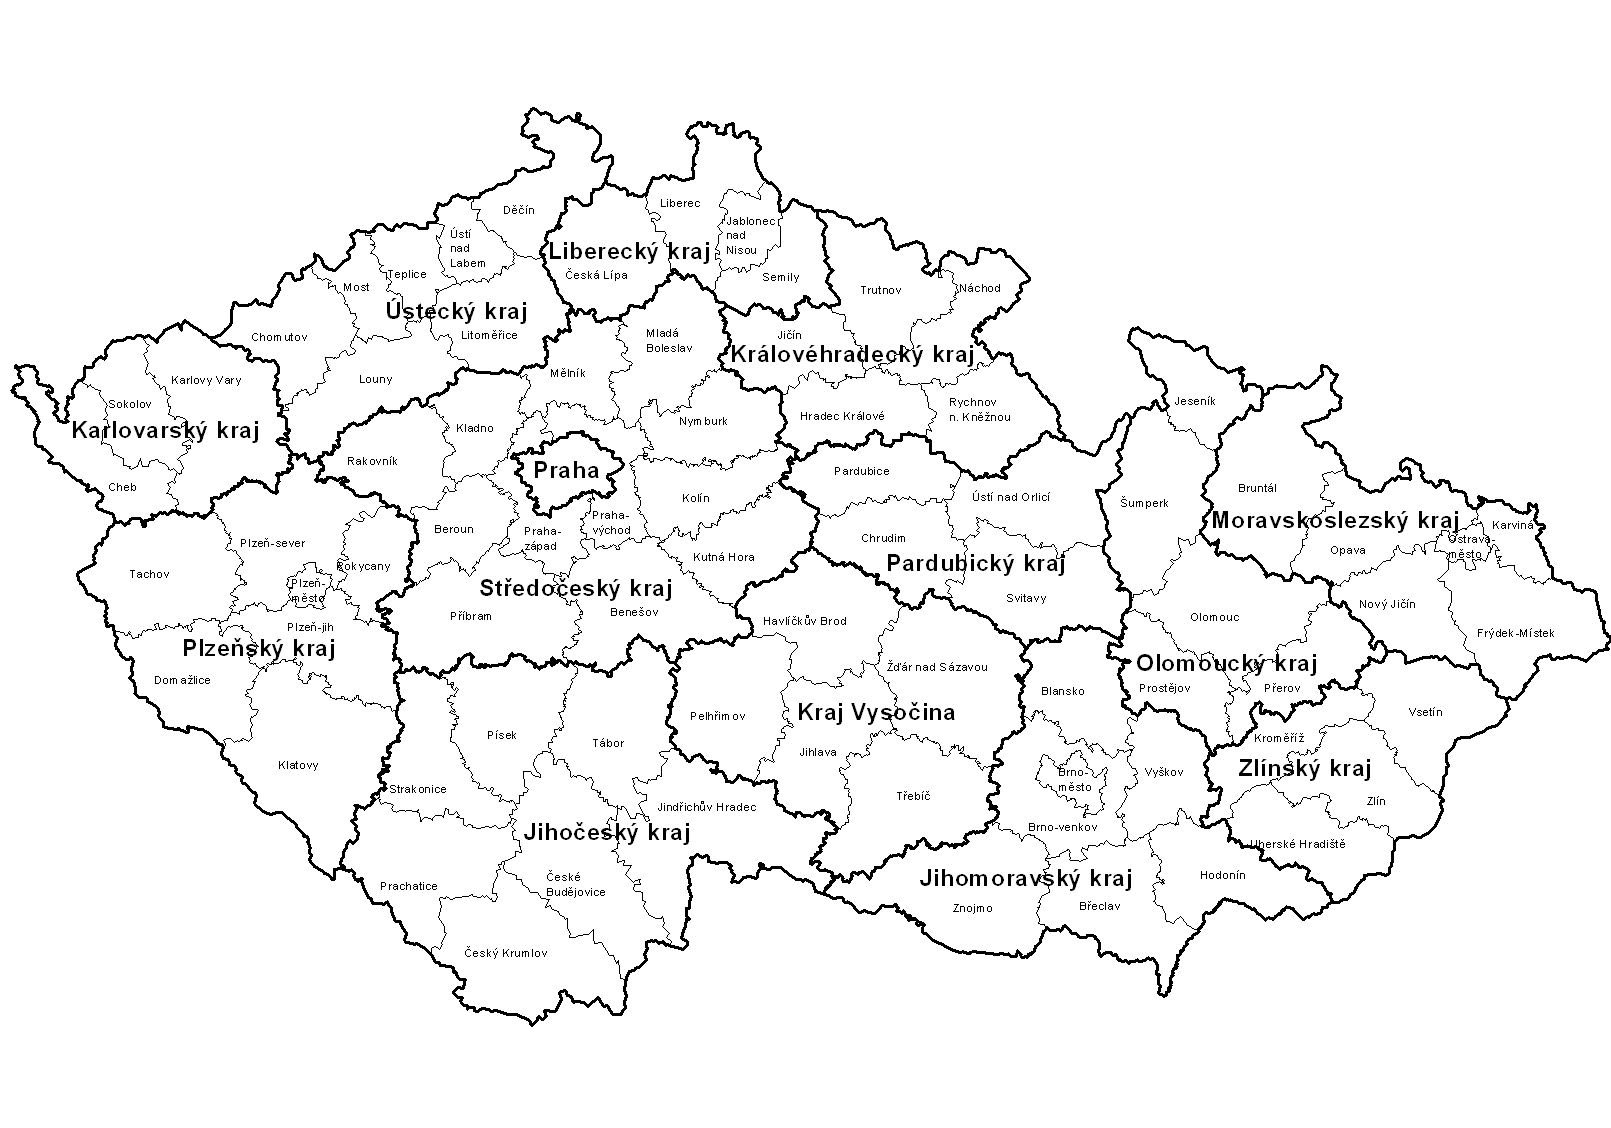
\includegraphics[width=\textwidth]{polit.jpg}
  \centering
  \caption{Political map of Czechia, via \href{http://www.mapaceskerepubliky.cz/mapa-kraju/}{www.mapaceskerepubliky.cz/mapa-kraju}}
\end{figure}

The top-level denomination are the 14 regions (Czech: kraje) and the second-level denomination are the 76 districts (Czech: okresy) – these are usually named after their biggest town/city. 

Most of Czech lanscape consists of rolling hills, making it somewhat similar to Germany or France in that sense. The country's borders consist for the most part of more mountanious areas.  

\begin{figure}[H]
  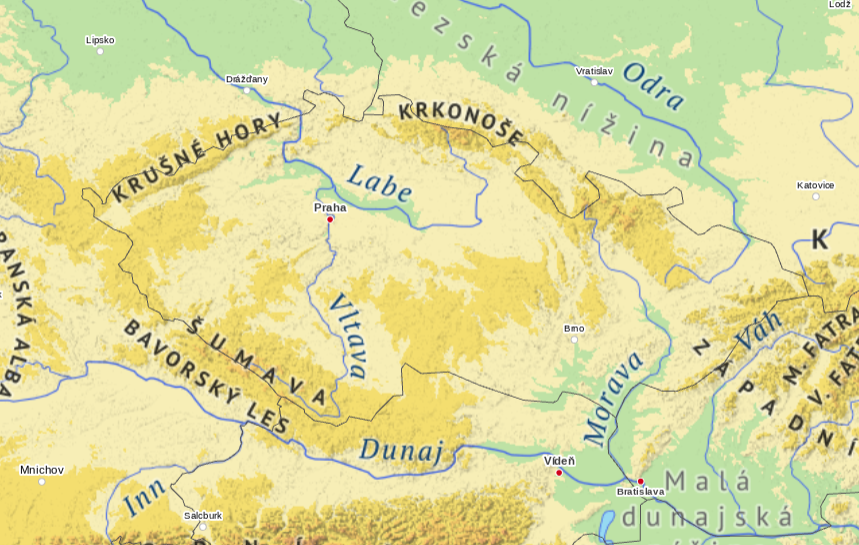
\includegraphics[width=\textwidth]{topo.png}
  \centering
  \caption{Topographic map of Czechia and surroundings, via \href{https://atlas.mapy.cz/}{atlas.mapy.cz}}
\end{figure}

In these ways it also differes from Poland and Slovakia. There are very few places within Czechia that can be dead-flat. These include a portion of the Jihočeský region (mainly in České Budějovice district), parts of the Elbe (Czech: Labe) plains as well as the parts of Jihomoravský region. None of these flatlands are particularly big or vast. On the contrary, Slovakia is (if we exclude the far-east part) either dead flat (near Bratislava) or highly mountanious. Poland is mostly dead-flat, other than for the regions at its southern flank, which get particularly mountanious. 

To distinguish Czechia from the aforementioned countries that have very similar rolling-hill landscape like France or Germany, refer to external sources, for example their respective plonkit entries (links: \href{https://www.plonkit.net/germany}{Germany}, \href{https://www.plonkit.net/france}{France}).

\subsection{Camera generation \& Copyright}

\subsection{Road markings}

\subsection{Bollards}

\subsection{Signs}

\subsection{Chevrons}

\subsection{Trail markings}

\subsection{Poles}


\newpage
\section{Region-guessing the country}

\newpage
\section{Acknowledgements}
\label{sec:ack}

\subsection{External graphics}

This document's graphics are incorporated partially from external sources. Special thanks goes to them, wherever they may be. The following is their list:

\begin{itemize}
  \item Title page Czechia map\cite{gr1}
\end{itemize}

\subsection{Contribees}


% =======================================================================
%
%                                BIBLIOGRAPHY
%
% =======================================================================

\newpage

\begin{thebibliography}{e}
\bibitem{gr1}
Flag-map of the Czech Republic. "Stasyan117." 2015. \textit{Wikimedia.org}. Wikimedia Commons. Web. 16 September 2024.


\end{thebibliography}

\end{document}
